% chapter_14_15_16.tex
% GTAC 2026 double-blind submission
% Content: Voice AI ecosystem convergence and AMD's missing opportunities (§14-16)

\documentclass[blind]{gtac}

\usepackage{cite}
\usepackage{xcolor}
\usepackage{booktabs}
\usepackage{tikz}
\usetikzlibrary{arrows.meta,positioning}
\usepackage[colorlinks=true, linkcolor=blue, urlcolor=blue, citecolor=blue]{hyperref}
\Urlmuskip=0mu plus 1mu\relax % allow long URLs in references to break

\SetWatermarkScale{0.3}
\SetWatermarkAngle{30}
\SetWatermarkColor{gray!20}

\title{{Physical AI and Vertical Sotware: Bridging the AMD's Softpower Gap - from the Voice AI Lens}}

\author{Anonymous}

\begin{document}

\maketitle

\pagestyle{fancy}
\fancyhf{}
\cfoot{\thepage}
\renewcommand{\headrulewidth}{0pt}
\chead{{\sffamily\textcolor{red}{\fontsize{10}{12}\selectfont\textbf{DO NOT FORWARD -- FOR GTAC'26 REVIEW COMMITTEE ONLY}}}}
\thispagestyle{fancy}

\begin{abstract}
The voice AI market, projected to reach \$47.5B by 2034 at a 35\% CAGR, has converged on a five-layer inference pipeline orchestrated by three dominant open-source frameworks: LiveKit Agents, Pipecat, and TEN. Within this convergence, NVIDIA has secured the hardware default not through silicon superiority alone but through \textbf{softpower}---a layered ecosystem surface of pre-packaged NIM inference containers, official framework integrations across LangChain, LlamaIndex, Pipecat, and LiveKit, domain-specific voice SDKs (Riva, Maxine, ACE), an embedded AI edge platform (Jetson), and cloud marketplace presence across Azure, AWS, and GCP. AMD holds a demonstrable structural inference advantage---34\% lower cost-per-token for 70B-class LLMs on MI300X versus H100, and single-GPU fit (192\,GB HBM3) for models that otherwise require two H100s---yet this advantage remains unrealized because AMD is absent from the ecosystem positions that determine the hardware default before a developer ever consciously selects compute. This paper uses the voice AI stack as a lens to map AMD's softpower gap across five downstream layers (framework plugin slots, serving infrastructure, voice-domain SDKs, edge hardware, cloud marketplace) and four upstream barriers (training and fine-tuning toolchain, ISV and systems-integrator channel, voice-plus-vision convergence, synthetic data for low-resource languages). We argue the bridge is already being built: Physical AI vertical software delivery---converting AMD model outputs into production pipelines and devkits for real customer deployments---is organically producing the same assets that close the ecosystem gap: a unified inference SDK, accelerated multi-modal pipelines, and a Jetson-class embedded devkit. The softpower gap is not unique to voice AI---the same pattern appears in robotics, industrial inspection, and healthcare imaging, making this analysis generalizable across AMD's physical AI investment areas.
\end{abstract}

\keywords{ROCm, MI300X, voice AI, ecosystem strategy, NIM, Pipecat, LiveKit, LangChain, inference, on-premise, DPDP, Riva.}

%---------------------------------------------------------------------------
\section{Introduction}
\label{sec:intro}
%---------------------------------------------------------------------------

Voice AI agents answer phones, qualify leads, triage patients, and run collections at a unit cost of approximately \$0.40 per call---one to two orders of magnitude below a human agent at \$7--\$12 per call~\cite{assemblyai_2026,grandview}. Production deployments grew 340\% year-over-year across 500+ organizations, and 80\% of customer-service organizations plan a voice AI deployment by end of 2026~\cite{assemblyai_2026}. Unlike model training, a deployed voice agent is a \emph{steady-state inference machine}: it does not train; it transcribes, reasons, and speaks 24 hours a day. At scale its dominant operating cost is GPU compute.

AMD's MI300X delivers a 34\% lower cost-per-token for LLM inference than the NVIDIA H100, and fits 70B-class models that otherwise require two H100s onto a single 192\,GB device. These advantages are real and compound at the scale voice AI platforms operate---a deployment handling 1M minutes/month can save approximately \$84K/month on LLM inference alone~\cite{spheron_rocm,vllm_rocm}. Yet AMD is largely absent from voice AI production deployments, not because its silicon is insufficient, but because the ecosystem surface through which developers and enterprises \emph{select} compute has been staked out by NVIDIA at every layer above the silicon.

This paper makes three contributions. First, we characterize the voice AI stack as a converging system---five layers, three frameworks, one critical hardware decision point---and explain how NVIDIA constructed its ecosystem position through the NIM (NVIDIA Inference Microservices) strategy (Sections~\ref{sec:stack}--\ref{sec:nim}). Second, we map AMD's current ROCm coverage per layer and then enumerate the complete set of ecosystem gaps across five downstream layers and four upstream barriers (Sections~\ref{sec:amd_today}--\ref{sec:upstream}). Third, we translate the full gap map into a prioritized action roadmap with engineering effort and business impact estimates (Sections~\ref{sec:gateway}--\ref{sec:roadmap}). The paper is self-contained so that a reader unfamiliar with the 2026 voice AI ecosystem can follow both the technical analysis and the strategic rationale.

%---------------------------------------------------------------------------
\section{The Voice AI Stack and Its Convergence}
\label{sec:stack}
%---------------------------------------------------------------------------

\subsection{Five Layers, Three Compute-Bearing}

A voice AI conversation traverses five distinct layers (Figure~\ref{fig:pipe}). The 2026 production end-to-end latency median is 680\,ms; the emerging bar is sub-500\,ms, which is especially tight on Indian cellular networks that add \texttt{\textasciitilde}50\,ms overhead over fiber~\cite{assemblyai_stack}.

\begin{figure}[t]
\centering
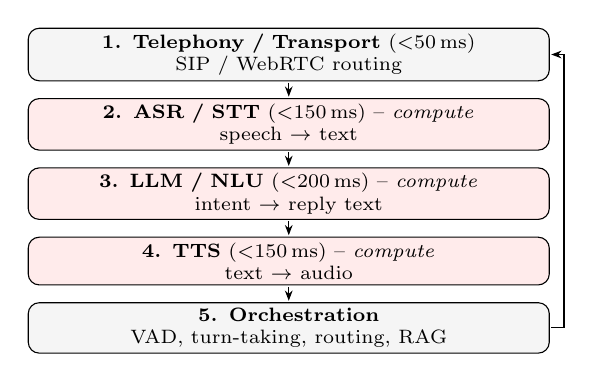
\begin{tikzpicture}[
  font=\scriptsize,
  box/.style={draw, rounded corners, align=center, text width=2.55in,
              minimum height=2.6ex, inner sep=2pt},
  comp/.style={box, fill=red!8},
  light/.style={box, fill=gray!8},
  arr/.style={-{Stealth[length=1.3mm]}, shorten >=0.5pt, shorten <=0.5pt}
]
\node[light] (tel) {\textbf{1. Telephony / Transport} ($<$50\,ms)\\ SIP / WebRTC routing};
\node[comp, below=1.4ex of tel] (asr)
  {\textbf{2. ASR / STT} ($<$150\,ms) -- \emph{compute}\\ speech $\rightarrow$ text};
\node[comp, below=1.4ex of asr] (llm)
  {\textbf{3. LLM / NLU} ($<$200\,ms) -- \emph{compute}\\ intent $\rightarrow$ reply text};
\node[comp, below=1.4ex of llm] (tts)
  {\textbf{4. TTS} ($<$150\,ms) -- \emph{compute}\\ text $\rightarrow$ audio};
\node[light, below=1.4ex of tts] (orc)
  {\textbf{5. Orchestration}\\ VAD, turn-taking, routing, RAG};
\draw[arr] (tel) -- (asr);
\draw[arr] (asr) -- (llm);
\draw[arr] (llm) -- (tts);
\draw[arr] (tts) -- (orc);
\draw[arr] (orc.east) -- ++(0.18,0) |- (tel.east);
\end{tikzpicture}
\caption{The five-layer voice pipeline with per-layer latency budget. Shaded layers
(ASR, LLM, TTS) are GPU-compute-bearing; AMD's hardware advantage and ecosystem
gaps both reside here.}
\label{fig:pipe}
\end{figure}

Telephony and orchestration are I/O- and control-bound and carry little GPU cost. ASR, LLM, and TTS consume GPU cycles per conversation. Counterintuitively, LLM inference is the cheapest of the three per minute but the most latency-critical---it must emit its first token in under 200\,ms. TTS is the \emph{hidden budget killer}: premium hosted synthesis costs \$0.10--\$0.30 per minute, which can exceed ASR and LLM combined, making self-hosted GPU-resident TTS economically critical at scale~\cite{bentoml_tts}.

\subsection{Three Frameworks Now Orchestrate Everything}

Despite hundreds of voice AI companies and billions in funding, production code has converged on three open-source orchestration frameworks. Commercial platforms---Vapi, Retell AI, Bolna, Caller Digital, Gnani, PolyAI, Synthflow---are business layers above one of:

\begin{itemize}
  \item \textbf{LiveKit Agents} (Apache 2.0)---the WebRTC backbone that OpenAI ChatGPT Voice Mode, Character.ai, and Meta all use. Native SIP integration shipped in 2025 so no Twilio bridge is required. Multi-participant, Model Context Protocol (MCP) tool support, full media server + agent SDK under one license.
  \item \textbf{Pipecat} (BSD-2, Daily.ai, v1.0 April 2026)---a Python frame-pipeline framework with 60+ service connectors covering every commercial ASR, LLM, TTS, and transport combination. Each audio frame flows through swappable VAD, STT, LLM, and TTS processors; changing providers requires no code rewrite. Ships with OpenTelemetry observability.
  \item \textbf{TEN Framework} (C++/Go/Python)---the highest-performance option because its core is C++, not Python. Includes proprietary VAD and turn-detection models optimized for sub-300\,ms response. Integrates avatar lip-sync (Trulience, HeyGen, Tavus) and includes a visual no-code editor for agent wiring.
\end{itemize}

Figure~\ref{fig:convergence} maps this convergence. Every commercial platform is a business layer above one of the three frameworks, which in turn share a common model layer. The GPU compute layer is the single point where AMD's hardware advantage and its ecosystem gap both reside: win there---or at the framework plugin layer immediately above---and the hardware choice is made for every platform above.

\begin{figure}[t]
\centering
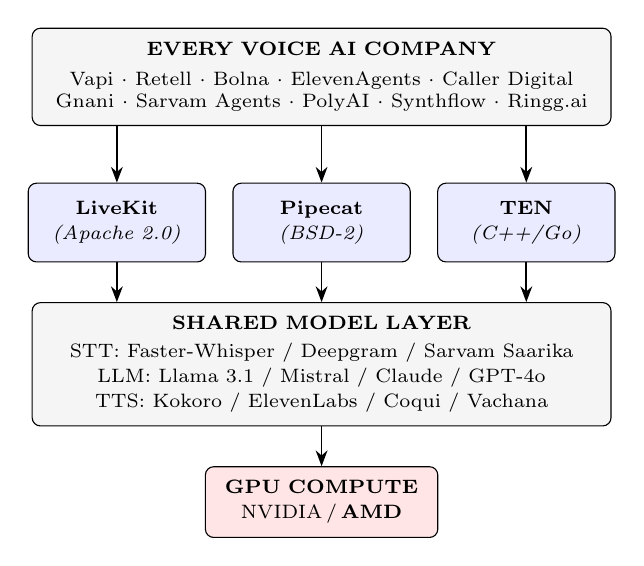
\begin{tikzpicture}[
  font=\scriptsize,
  topbox/.style={draw, rounded corners=3pt, fill=gray!8,
                 text width=7.0cm, align=center, inner sep=5pt},
  fwbox/.style={draw, rounded corners=3pt, fill=blue!8,
                text width=1.9cm, align=center, inner sep=5pt,
                minimum height=1.0cm},
  midbox/.style={draw, rounded corners=3pt, fill=gray!8,
                 text width=7.0cm, align=center, inner sep=5pt},
  gpubox/.style={draw, rounded corners=3pt, fill=red!10,
                 text width=2.6cm, align=center, inner sep=5pt},
  arr/.style={-{Stealth[length=2mm]}, semithick}
]
%--- Row 1: every voice AI company -----------------------------------------
\node[topbox] (top) at (0,0) {%
  \textbf{EVERY VOICE AI COMPANY}\\[3pt]
  Vapi $\cdot$ Retell $\cdot$ Bolna $\cdot$ ElevenAgents $\cdot$ Caller Digital \\
  Gnani $\cdot$ Sarvam Agents $\cdot$ PolyAI $\cdot$ Synthflow $\cdot$ Ringg.ai%
};
%--- Row 2: three frameworks ------------------------------------------------
\node[fwbox] (livekit) at (-2.6,-1.85) {%
  \textbf{LiveKit}\\[1pt]\textit{(Apache 2.0)}%
};
\node[fwbox] (pipecat) at ( 0.0,-1.85) {%
  \textbf{Pipecat}\\[1pt]\textit{(BSD-2)}%
};
\node[fwbox] (ten)     at ( 2.6,-1.85) {%
  \textbf{TEN}\\[1pt]\textit{(C++/Go)}%
};
%--- Row 3: shared model layer ----------------------------------------------
\node[midbox] (model) at (0,-3.65) {%
  \textbf{SHARED MODEL LAYER}\\[2pt]
  STT: Faster-Whisper / Deepgram / Sarvam Saarika\\[1pt]
  LLM: Llama 3.1 / Mistral / Claude / GPT-4o\\[1pt]
  TTS: Kokoro / ElevenLabs / Coqui / Vachana%
};
%--- Row 4: GPU compute layer -----------------------------------------------
\node[gpubox] (gpu) at (0,-5.4) {%
  \textbf{GPU COMPUTE}\\[1pt]NVIDIA\,/\,\textbf{AMD}%
};
%--- Arrows: top -> frameworks ----------------------------------------------
\draw[arr] (livekit.north |- top.south) -- (livekit.north);
\draw[arr] (pipecat.north |- top.south) -- (pipecat.north);
\draw[arr] (ten.north     |- top.south) -- (ten.north);
%--- Arrows: frameworks -> model layer -------------------------------------
\draw[arr] (livekit.south) -- (livekit.south |- model.north);
\draw[arr] (pipecat.south) -- (pipecat.south |- model.north);
\draw[arr] (ten.south)     -- (ten.south     |- model.north);
%--- Arrow: model -> GPU compute --------------------------------------------
\draw[arr] (model.south) -- (gpu.north);
\end{tikzpicture}
\caption{Voice AI industry convergence: every commercial platform is a business layer
  above one of three open-source orchestration frameworks (LiveKit Agents, Pipecat, TEN),
  which share a common model layer (STT, LLM, TTS). The GPU compute layer at the bottom
  is where AMD's hardware advantage resides and where ecosystem positioning determines
  which vendor becomes the default substrate for all platforms above.}
\label{fig:convergence}
\end{figure}

%---------------------------------------------------------------------------
\section{CUDA Gap Closed; AMD Still Lacks a Low-Resistance Path to Its Silicon}
\label{sec:amd_today}
%---------------------------------------------------------------------------

Table~\ref{tab:compat} summarizes AMD's current ROCm coverage across the voice AI compute stack. The pattern is clear: the two heaviest compute layers (LLM serving and TTS synthesis) are solved; two narrower but load-bearing pieces---streaming ASR and HuggingFace Text Embeddings Inference (TEI) for RAG-augmented agents---remain open.

\begin{table}[t]
\centering
\caption{ROCm support for voice-AI components (2026).}
\label{tab:compat}
\footnotesize
\begin{tabular}{@{}lll@{}}
\toprule
Component & ROCm & Note \\
\midrule
LLM serving (vLLM, Llama 3.1) & Full & 90--95\% of H100 throughput \\
LLM serving (SGLang) & Full & Within 5--10\% of CUDA \\
TTS: Kokoro, Chatterbox & Full & Pure PyTorch, zero changes \\
TTS: Coqui XTTS-v2 & Partial & Works with effort \\
ASR: Faster-Whisper (batch) & Full & Real-time mode needs extra work \\
ASR: streaming containers & \textbf{Gap} & CUDA-assumed ecosystem \\
Embeddings: HF TEI & \textbf{Gap} & No ROCm build available \\
\bottomrule
\end{tabular}
\end{table}

\textbf{LLM layer: structural CapEx and cost-per-token advantage.}
Table~\ref{tab:llm} shows MI300X delivering comparable throughput at substantially lower hourly cost, yielding a 34\% lower cost per million tokens. The VRAM result is structural rather than incremental: a 70B-class model requires two H100s (160\,GB combined) but fits on a single MI300X, halving node count and removing the NVLink/interconnect complexity. On MLPerf Inference v6.0, MI355X (288\,GB HBM3e) landed within single-digit percentage points of B200 on server inference workloads~\cite{mlperf6}.

\begin{table}[t]
\centering
\caption{LLM inference: MI300X vs.\ H100 SXM5 (2026 figures).}
\label{tab:llm}
\footnotesize
\begin{tabular}{@{}lcc@{}}
\toprule
Dimension & MI300X & H100 SXM5 \\
\midrule
VRAM & \textbf{192\,GB} HBM3 & 80\,GB HBM3e \\
On-demand cloud price & \$1.50--2.50/hr & \$2.90/hr \\
Throughput (tok/s, Llama 3.1 70B) & \texttt{\textasciitilde}18{,}000 & \texttt{\textasciitilde}19{,}500 \\
Cost / 1M tokens & \textbf{\$0.027} & \$0.041 \\
70B fits on 1 GPU? & \textbf{Yes} & No (needs 2) \\
\bottomrule
\end{tabular}
\end{table}

\textbf{TTS layer: pure PyTorch runs unmodified.}
The leading self-hostable TTS models---Kokoro (82\,M parameters, Apache 2.0), Chatterbox, and Coqui XTTS-v2---are pure PyTorch and run on ROCm without source changes because HIP transparently maps CUDA calls~\cite{bentoml_tts}. For any operator self-hosting TTS to avoid \$0.10--\$0.30/min hosted pricing, AMD is already a viable cost-competitive target with no porting effort.

\textbf{What AMD is missing.}
Despite competitive silicon, AMD is absent from the ecosystem surface that drives the adoption decision. Table~\ref{tab:nim_gap} shows the NIM-layer gap: ten ecosystem positions where NVIDIA is present and AMD is not. The gap is not silicon; it is containers, plugins, blueprints, and marketplace slots.

\begin{table}[t]
\centering
\caption{NIM ecosystem gap: NVIDIA current vs.\ AMD required.}
\label{tab:nim_gap}
\footnotesize
\begin{tabular}{@{}lll@{}}
\toprule
NVIDIA Has & AMD Equivalent & Status \\
\midrule
Riva ASR NIM container & AMD-certified ASR container & \textbf{Absent} \\
Riva TTS NIM container & AMD-certified TTS container & \textbf{Absent} \\
AI Blueprint: voice agent (global) & AMD Blueprint: Pipecat on MI300X & \textbf{Absent} \\
AI Blueprint: India voice & AMD Blueprint: Sarvam on MI300X & \textbf{Absent} \\
Pipecat official NVIDIA processor & Pipecat official AMD processor & \textbf{Absent} \\
LiveKit certified GPU backend & LiveKit AMD-certified backend & \textbf{Absent} \\
VS Code NIM extension & VS Code ROCm / AMD Quark extension & \textbf{Absent} \\
Azure Foundry NIM (July 2026) & Azure AMD inference endpoint & Partial \\
SI certification (TCS, Infosys...) & India SI certification program & \textbf{Absent} \\
28M developers defaulting to CUDA & AMD developer default & Opt-in only \\
\bottomrule
\end{tabular}
\end{table}

%---------------------------------------------------------------------------
\section{How NVIDIA Became the Hardware Gateway: The NIM Playbook}
\label{sec:nim}
%---------------------------------------------------------------------------

NVIDIA's dominance was not achieved through silicon alone. The decisive instrument was the \textbf{NIM (NVIDIA Inference Microservices)} platform: pre-packaged, production-ready containers that make NVIDIA silicon the path of least resistance at the first developer touchpoint. For voice AI specifically, the NIM strategy delivers:

\begin{enumerate}
  \item \textbf{Riva ASR NIM}---a ready-to-run streaming ASR microservice (Parakeet TDT model) deployable with a single \texttt{docker pull}. No model configuration, no streaming pipeline assembly, no VAD tuning.
  \item \textbf{Maxine Studio Voice NIM}---real-time noise suppression and acoustic echo cancellation as a gRPC microservice. Directly improves ASR word error rate (WER) in noisy call center environments.
  \item \textbf{AI Blueprints}---complete, deployable voice agent applications (not documentation). Teams clone and adapt. The GPU choice is already encoded in the Blueprint.
  \item \textbf{RTX Spark}---a Grace+Blackwell module with 128\,GB shared CPU/GPU memory for on-device developer use. The developer who prototypes on RTX Spark defaults to NVIDIA in production.
  \item \textbf{Azure AI Foundry native NIM integration} (July 2026)---deploy to cloud from VS Code with one click, NVIDIA GPU underneath.
  \item \textbf{SI certification program}---TCS, Infosys, Wipro, Accenture, and Capgemini are formally certified NIM implementation partners; their delivery playbooks, pre-sales demos, and engineer training all reference NVIDIA tooling.
\end{enumerate}

The result: when a developer follows an AI Blueprint for a voice agent, they never consciously select a GPU---the choice is already made. NVIDIA is the default. Every other choice requires active effort.

%---------------------------------------------------------------------------
\section{The Five Downstream Ecosystem Layers}
\label{sec:downstream}
%---------------------------------------------------------------------------

NVIDIA's ecosystem position spans five distinct downstream layers. Each operates on the same logic: ship a named package, container, or SDK; let developers adopt it as the default; the hardware choice becomes invisible at the call site.

\subsection{Layer 1 --- Framework Plugin Slots}

\begin{table}[t]
\centering
\caption{Framework ecosystem presence.}
\label{tab:framework}
\footnotesize
\begin{tabular}{@{}lll@{}}
\toprule
Framework & NVIDIA & AMD \\
\midrule
Pipecat & Official processor plugin & Absent \\
LiveKit Agents & Certified GPU backend & Absent \\
LangChain & \texttt{langchain-nvidia-ai-endpoints} & Absent \\
LlamaIndex & \texttt{llama-index-llms-nvidia} & Absent \\
Haystack & NIM native pipeline component & Absent \\
\bottomrule
\end{tabular}
\end{table}

Every LangChain or LlamaIndex voice agent that uses NIM routes to NVIDIA hardware at the endpoint level. The developer writes \texttt{ChatNVIDIA(model="{...}")}---done. AMD does not exist at that call site. The same call, repeated across millions of agent pipelines, is the mechanism by which NVIDIA becomes the default GPU substrate for every voice AI application built in 2025--2026.

\subsection{Layer 2 --- Inference Serving Infrastructure}

\textbf{NVIDIA Triton / Dynamo-Triton} is the invisible substrate beneath every production voice pipeline. ASR, LLM, and TTS models are all served from Triton with disaggregated LLM serving (prefix caching, KV offload). Users include Microsoft, American Express, Salesforce, Naver, and Hugging Face. It runs inside AWS SageMaker, Azure Machine Learning, Google Vertex AI, and Oracle Cloud.

\textbf{TensorRT-LLM} sits on top of Triton. At batch size 1--4 (real-time voice, latency-critical), TensorRT-LLM holds a 20--30\% throughput advantage over vLLM ROCm. For voice fleets this is the latency gap that matters: a 50\,ms difference in LLM token generation is audible to a human ear.

AMD's position: vLLM ROCm became officially first-class in January 2026, with CI pass rate jumping from 37\% in November 2025 to 93\% in six weeks and the first pre-built Docker image shipping~\cite{vllm_rocm}. This is genuine progress. But vLLM is one serving tool; Triton is infrastructure. There is no AMD model serving standard with multi-model ensemble orchestration, no AMD equivalent of Dynamo's disaggregated serving, and no AMD inference server that a Fortune 500 enterprise would treat as an equivalent drop-in.

\subsection{Layer 3 --- Voice-Domain SDKs}

NVIDIA ships three domain-specific SDKs for voice AI. Each pulls Triton and TensorRT as dependencies, creating a complete vertical stack from model artifact to production microservice.

\textbf{NVIDIA Riva}---full conversational AI SDK: ASR + TTS + neural machine translation + speaker diarization + speaker identification + VAD, served as gRPC microservices with enterprise SLA. Fine-tunable on custom speech data via NVIDIA NeMo. Supports English plus eleven languages including Hindi, Arabic, Mandarin, and Spanish. Real-world deployment: the Caterpillar Cat AI Assistant runs Riva on a Jetson Thor module inside heavy construction machinery---obstacle detection, operator voice commands, and spoken response, entirely on-device with no cloud dependency.

\textbf{NVIDIA Maxine}---audio and video enhancement SDK: real-time noise suppression, acoustic echo cancellation, room reverb removal. For voice AI in call centers, noise suppression before ASR is not optional---it is the difference between 10\% and 25\% WER in a noisy environment~\cite{whisper_wer}. Integrated into Cisco and Zoom.

\textbf{NVIDIA ACE (Avatar Cloud Engine)}---digital human platform: Riva (voice) + Audio2Face (lip-sync from audio) + Nemotron LLM (dialogue) + P-Flow voice cloning from 30 minutes of audio, all as NIM microservices. Partners include Convai, Inworld, and UneeQ. Deployed in customer service kiosks, retail concierges, healthcare reception, and gaming NPCs.

AMD has no equivalent for any of the three. A hospital kiosk or bank branch digital concierge built on ACE is locked to NVIDIA at every layer---not by contract, but by the absence of any AMD-equivalent component.

\subsection{Layer 4 --- Edge Hardware Platform}

\textbf{NVIDIA Jetson} is the dominant embedded AI compute platform: hardware modules ranging from Jetson Nano (\texttt{\textasciitilde}\$100) to Jetson AGX Orin (64\,GB, 275\,TOPS) to Jetson Thor (next-gen, 241\,TOPS with MIG support). JetPack OS ships with Riva, vLLM, NemoClaw agentic framework, and the full CUDA stack. Certified OEM partners include ADLINK, Siemens, and KUKA, covering retail kiosks, smart factory floor copilots, autonomous mobile robots, agricultural drones, and in-vehicle assistants.

The Caterpillar deployment is the clearest signal: Jetson Thor + Riva ASR (Nemotron speech models) + Qwen3 4B via vLLM, running entirely on-device inside a bulldozer cab. This is the template for embedded voice AI across heavy industry, healthcare, and automotive.

AMD's answer: the Ryzen AI NPU runs Whisper BFP16 locally on a laptop and is documented~\cite{amd_ryzen_whisper}. It works. But there is no industrial edge module, no JetPack-equivalent OS image, no certified hardware partners for robotics or kiosk deployment, no AMD reference design for an offline factory floor voice copilot. The Ryzen AI NPU addresses the developer laptop; Jetson addresses every physical deployment. Only NVIDIA is present in the physical deployment market.

\subsection{Layer 5 --- Cloud Marketplace Slots}

\begin{table}[t]
\centering
\caption{Cloud marketplace GPU presence.}
\label{tab:cloud}
\footnotesize
\begin{tabular}{@{}lll@{}}
\toprule
Platform & NVIDIA & AMD \\
\midrule
Azure AI Foundry & NIM native (July 2026) & Absent \\
HF Inference Endpoints & T4, A10G, A100, H100 selectable & Not selectable$^{*}$ \\
AWS SageMaker & Triton + NIM containers & Limited \\
Google Vertex AI & Triton available & Limited \\
Oracle Cloud AI & Triton available & Absent \\
\bottomrule
\multicolumn{3}{l}{$^{*}$TGI ROCm Docker image is production-ready but not surfaced in the UI.}
\end{tabular}
\end{table}

The HuggingFace Inference Endpoints gap is the sharpest illustration. AMD has a formal hardware partnership with HuggingFace. The TGI ROCm Docker image is production-ready and validates MI210, MI250, and MI300X with Flash Attention 2, AWQ quantization, and DeepSpeed. The engineering is done. But when a developer opens the HF Inference Endpoints UI and clicks ``deploy this Whisper model'' or ``deploy this Llama model,'' MI300X does not appear in the GPU dropdown---NVIDIA T4 through H100 does. The developer selects NVIDIA, not because AMD cannot run the model, but because AMD is not on the menu.

That is the ecosystem gap in its simplest form: not a silicon gap, but a \emph{slot gap}.

%---------------------------------------------------------------------------
\section{The Four Upstream Gaps}
\label{sec:upstream}
%---------------------------------------------------------------------------

The downstream gaps (Section~\ref{sec:downstream}) are visible, concrete, and closeable. The upstream gaps operate before a model is deployed, before a developer picks a framework, and before an enterprise issues a purchase order. Closing only the downstream gaps puts AMD in contention for inference workloads. Closing the upstream gaps creates platform momentum.

\subsection{Gap 1 --- The Training and Fine-Tuning Moat}

Voice AI companies do not merely serve pre-trained models. They fine-tune on proprietary data continuously: custom ASR acoustic models trained on their customers' speech (medical transcription, legal dictation, financial advisory), custom TTS voice clones trained to a brand's voice persona, custom NLU models for domain-specific intents. This fine-tuning loop runs weekly or monthly in production and is entirely NVIDIA-anchored.

\textbf{NVIDIA NeMo} is the training and fine-tuning framework purpose-built for speech and language models. It provides recipes for ASR fine-tuning (Conformer, Parakeet), TTS voice cloning (FastPitch, HiFi-GAN), and LLM instruction tuning, with Triton export as the final step. A company that fine-tunes a Riva ASR model using NeMo obtains a TensorRT-optimized artifact that deploys directly to Triton: from raw audio to production microservice in one command.

Critical fine-tuning libraries are CUDA-primary on AMD (Table~\ref{tab:finetune}).

\begin{table}[t]
\centering
\caption{Fine-tuning library gaps on AMD ROCm.}
\label{tab:finetune}
\footnotesize
\begin{tabular}{@{}lll@{}}
\toprule
Library & Role & AMD ROCm Status \\
\midrule
\texttt{bitsandbytes} & 4-bit / 8-bit quantization & Community fork only \\
\texttt{trl} (HuggingFace) & RLHF and fine-tuning framework & CUDA-primary; ROCm experimental \\
Axolotl & Most-used open fine-tuning tool & CUDA-primary; ROCm untested \\
PEFT & LoRA / QLoRA adapters & Works; less tested on AMD \\
FlashAttention 3 & Fastest attention kernel (Hopper) & No AMD equivalent \\
NVIDIA CUTLASS & High-perf CUDA kernel templates & AMD CK exists; smaller ecosystem \\
\bottomrule
\end{tabular}
\end{table}

The training moat creates inference lock-in. A model's artifact, optimization flags, quantization format, and deployment recipe are all NVIDIA-native; re-running fine-tuning on AMD costs engineering time with no revenue upside. Companies do not make this switch without a compelling external reason.

\subsection{Gap 2 --- The ISV and SI Sales Channel Moat}

Enterprises do not choose GPU vendors directly. They buy software from independent software vendors (ISVs) and deploy through systems integrators (SIs). The GPU is chosen implicitly by the ISV's architecture decision, made years before the enterprise procurement conversation.

Major ISV integrations NVIDIA holds in voice AI:
\begin{itemize}
  \item \textbf{Genesys} (11,000+ enterprise contact center customers)---NVIDIA GPU-backed real-time agent assist and post-call analytics.
  \item \textbf{Cisco Webex}---NVIDIA Maxine noise suppression baked into the product; not a feature toggle, it is the product.
  \item \textbf{Salesforce Einstein Voice}---NVIDIA inference backend for voice-to-CRM transcription and intent extraction.
  \item \textbf{ServiceNow Now Assist}---NVIDIA NIM backend for voice-triggered workflow automation.
  \item \textbf{Five9, NICE CXone, Avaya}---contact center platforms with NVIDIA integrations.
\end{itemize}

AMD has no presence in any major contact center ISV platform. When an enterprise selects Genesys or Cisco Webex, AMD is not in the conversation---the GPU vendor was selected when Genesys chose its AI stack.

NVIDIA's formally certified SI partners---TCS, Infosys, Wipro, Accenture, and Capgemini---now sell NVIDIA-based voice AI to Fortune 500 clients as a packaged offering. Their engineers are trained on NVIDIA tooling, their delivery playbooks reference it, their pre-sales demos run on it. A client asking for AMD would require the SI to rebuild its practice from scratch. Without SI certification, AMD hardware will not appear in enterprise voice AI bids regardless of technical merit.

\subsection{Gap 3 --- Voice Plus Vision Convergence}

The next generation of deployed voice AI agents---retail kiosks, factory floor copilots, healthcare reception desks, in-vehicle assistants, delivery robots---combine voice with vision. A camera observes the environment; a microphone captures speech; the system integrates both to respond appropriately. NVIDIA offers a unified multi-modal stack:

\begin{itemize}
  \item \textbf{Jetson Thor} with Isaac (robotics vision + manipulation), Metropolis (video analytics), Riva (voice), and ACE (avatar)---all on a single CUDA substrate, one SDK, one vendor relationship.
  \item The Caterpillar Cat AI Assistant exemplifies the template: Jetson Thor + Isaac obstacle detection + Riva ASR + Qwen3 4B LLM + Riva TTS, entirely on-device inside a bulldozer cab.
\end{itemize}

When voice AI companies grow their product to include a camera---and they will, because vision context dramatically improves agent responses---they stay on NVIDIA because AMD has no landing zone. AMD's current product lines do not converge on a single device:

\begin{itemize}
  \item \textbf{MI300X}---data center inference; no vision pipeline.
  \item \textbf{Ryzen AI NPU}---laptop on-device inference; no industrial form factor.
  \item \textbf{Radeon GPUs}---graphics and gaming; separate driver stack, not integrated with ROCm.
\end{itemize}

No unified edge module. No multi-modal SDK bridging voice and vision on a single AMD device. This is a missing product category, not a missing library, and it requires a hardware roadmap decision rather than an engineering sprint.

\subsection{Gap 4 --- Synthetic Data for Low-Resource Languages}

Training high-quality ASR for low-resource languages requires synthetic speech data. Real transcribed audio in Hindi, Bengali, Tamil, Telugu, Swahili, or Filipino is scarce---not because the languages are rare, but because the recording and transcription infrastructure to produce training-grade data at scale has never been systematically built for these markets.

\textbf{NVIDIA's Nemotron} is a synthetic speech data generation pipeline that produces diverse, high-quality synthetic audio from text, including varied accents, speaking rates, background conditions, and speaker demographics. Sarvam AI, Gnani.ai, and AI4Bharat (IIT Madras)---the three organizations building India's voice AI language model foundation---all trained on NVIDIA DGX clusters using NVIDIA-native pipelines.

The consequence compounds: even if AMD wins an inference contract for a Sarvam-based voice agent, the Sarvam model was trained on NVIDIA. Its fine-tuning requires NVIDIA-compatible tooling; its next version will be trained on NVIDIA. The model's lifecycle is anchored to NVIDIA before it reaches a production AMD server. AMD has no synthetic speech data generation capability, no training compute partnership with AI4Bharat or Sarvam, and no AMD-sponsored voice dataset for Indian, African, or Southeast Asian languages~\cite{indic_asr,sarvam_asr}.

For the India BFSI opportunity (Section~\ref{sec:roadmap}), this matters enormously. India's 22 official languages represent a 1.4B-person market where model quality determines which company wins. Every model trained on NVIDIA infrastructure creates a training-data dependency that outlasts the initial compute decision.

%---------------------------------------------------------------------------
\section{The AMD Gateway Strategy}
\label{sec:gateway}
%---------------------------------------------------------------------------

The downstream gaps are closeable with bounded engineering effort. The strategic playbook is to execute what NVIDIA ran---but targeting the cost wedge that NVIDIA's pricing creates. At 1M minutes/month, the LLM cost advantage alone is \$84K/month~\cite{spheron_rocm,vllm_rocm}; self-hosted ROCm TTS eliminates an additional \$100K--\$300K/month in hosted synthesis costs; and India on-premise deployments benefit from \texttt{\textasciitilde}50\% lower GPU CapEx. The pitch is straightforward: same Pipecat code, same LiveKit transport, 34\% lower per-conversation LLM cost.

\textbf{Step 1: Three certified containers.}
The developer test is: ``Does this run on AMD?'' If the answer is a single \texttt{docker pull} to a certified, benchmarked AMD container, it takes 30 seconds to validate. Three containers cover the critical use cases: (a) an AMD Pipecat Voice Agent container combining Faster-Whisper + vLLM (Llama 3.1 8B) + Kokoro TTS + Pipecat 1.0 + Silero VAD + LiveKit transport on ROCm 7.2; (b) an AMD LiveKit Voice Agent container with the same model stack and native SIP bridge; (c) an AMD Sarvam India Voice Agent container with Sarvam Saarika ASR + Sarvam Bulbul TTS + Llama 3.1 + Pipecat, with DPDP-compliant audit logging, running entirely on-premise.

\textbf{Step 2: AMD Voice AI Blueprints.}
Mirror NVIDIA's AI Blueprints: complete, deployable repos---not documentation. Each Blueprint ships as one \texttt{docker-compose.yml} and one Python entry point. Target markets: US/EU enterprise contact center (Pipecat + Faster-Whisper + Llama 3.1 70B + Kokoro), India BFSI (LiveKit + Sarvam Saarika + Sarvam-30B + Vachana TTS), Arabic GCC banking, edge/offline India (Ryzen AI NPU + Whisper Small + Llama 3.2 3B + Kokoro---no GPU, no cloud, no API key, DPDP-compliant). Critical: Blueprints must also run on a consumer-grade AMD GPU (\texttt{\textasciitilde}\$700) to reach developers who cannot expense datacenter hardware.

\textbf{Step 3: ROCm plugin certification for Pipecat.}
An official \texttt{pipecat-ai[amd]} PyPI package that registers AMD-optimized Faster-Whisper, Kokoro, and vLLM serving as first-class Pipecat processors, appearing in Pipecat's official documentation as a supported compute backend. Estimated effort: two weeks. This positions AMD alongside Deepgram, ElevenLabs, and OpenAI as an official Pipecat integration partner.

\textbf{Step 4: HuggingFace TEI on ROCm.}
Upstream ROCm support into HuggingFace Text-Embeddings-Inference (TEI) closes the last meaningful software gap for enterprise voice agents using retrieval-augmented generation (RAG)---product catalogs, policy documents, FAQ databases. This is a bounded engineering project with a disproportionate ecosystem payoff.

\textbf{Step 5: HuggingFace Inference Endpoints slot.}
TGI ROCm is production-ready; AMD needs a commercial agreement with HuggingFace to make MI300X appear as a selectable GPU option in the Inference Endpoints UI. Zero engineering weeks. One business conversation. Immediate developer visibility across every model deployment that flows through HF Inference Endpoints---voice, LLM, embedding.

\textbf{Step 6: Ryzen AI NPU as developer on-ramp.}
AMD already publishes Whisper-on-NPU documentation~\cite{amd_ryzen_whisper}. The next step is a \texttt{pipecat create {-}{-}backend amd-npu} template that scaffolds a complete voice agent on Ryzen AI---Whisper Tiny on NPU, Llama 3.2 3B via Ollama, Kokoro TTS on CPU. No GPU required. No cloud required. No API key required. Runs offline. DPDP-compliant. This is the developer laptop demo that converts engineers into AMD advocates---the same role that RTX Spark plays for NVIDIA.

%---------------------------------------------------------------------------
\section{Prioritized Action Roadmap}
\label{sec:roadmap}
%---------------------------------------------------------------------------

Table~\ref{tab:roadmap} presents the full gap map with effort estimates across all ecosystem layers. The first group requires no new silicon, no new product categories, and no hardware roadmap decisions. The second group requires business development alongside engineering. The third group requires strategic hardware commitments and has a 2--3 year minimum horizon.

\begin{table}[t]
\centering
\caption{Prioritized AMD action roadmap across all ecosystem layers.}
\label{tab:roadmap}
\footnotesize
\begin{tabular}{@{}p{1.38in}p{0.62in}p{0.62in}p{0.52in}@{}}
\toprule
Action & Effort & Horizon & Impact \\
\midrule
HF Inference Endpoints slot & Business neg. & 0--4 wks & High \\
Certified ASR + TTS containers & 2 wks each & 1 month & High \\
Pipecat AMD processor (PyPI) & 2 wks & 1 month & Medium \\
LangChain / LlamaIndex / Haystack & 2--4 wks ea. & 1--2 months & High \\
AMD Voice AI Blueprints (4 targets) & 4 wks each & 2 months & High \\
\texttt{bitsandbytes} ROCm official & 4--6 wks & 2 months & High \\
Triton ROCm certified image & 12--16 wks & 4 months & High \\
Ryzen AI NPU voice template & 4 wks & 2 months & Medium \\
Genesys ISV integration & Business dev & 6--12 months & Very high \\
SI cert.\ program (TCS, Infosys...) & Program build & 6--12 months & Very high \\
AMD voice data initiative (India) & \$5--13M, 2 yr & 18--24 months & Strategic \\
FlashAttention 3 / CDNA3 equiv. & 16--24 wks & 6 months & Medium \\
Jetson-equiv.\ industrial edge module & HW roadmap & 2--3 years & Very high \\
\bottomrule
\end{tabular}
\end{table}

\textbf{The India BFSI beachhead.}
The cleanest near-term entry is markets where on-premise deployment is mandatory. India's Digital Personal Data Protection (DPDP) Act treats call audio as biometric data and constrains cross-border transfer, making cloud-only US-hosted stacks legally risky for banking, financial services, and insurance deployments~\cite{dpdp_checklist}. On-premise procurement is decided on CapEx, where AMD's \texttt{\textasciitilde}50\% lower GPU list price for equivalent capability is a direct advantage~\cite{india_guide}. India is the second-largest concentration of voice AI startups globally and a market projected to reach \$1B by 2030 (35.7\% CAGR)~\cite{slator_sarvam,india_guide}; sovereign-AI efforts there deploy on-premise by design. The AMD Sarvam Blueprint (Step 1c) targets this market directly, and the Ryzen AI NPU extends the data-residency story from datacenter to branch office~\cite{amd_ryzen_whisper}.

\textbf{ISV and SI leverage.}
Genesys alone reaches 11,000+ enterprise contact center customers. A single ISV integration gives AMD hardware presence in enterprise procurement conversations it currently never enters. The SI certification program is the demand-creation counterpart: once TCS or Infosys has certified AMD-based voice AI delivery playbooks, they surface AMD in bids proactively.

\textbf{The data initiative.}
An AMD-sponsored voice data initiative for high-priority markets---a partnership with AI4Bharat or a similar academic institution to fund transcription and annotation of 10,000+ hours of speech per language, with AMD compute provided for training---costs approximately \$5--13M over two years. The return: a voice model ecosystem that is AMD-native from inception, not ported from NVIDIA as an afterthought. For India's 22 official languages, this is the only path to structural influence over which hardware trains the models that serve 1.4B people~\cite{indic_asr,sarvam_asr}.

\textbf{First 12--16 weeks: what to do right now.}
Total engineering investment for Steps 1--4 (Section~\ref{sec:gateway}) is approximately 12--16 weeks for a focused team of six to eight engineers: three certified containers (six weeks), four AMD Voice AI Blueprints (eight weeks), one Pipecat PyPI plugin (two weeks), and HF TEI ROCm upstream (running in parallel). The HF Inference Endpoints slot closes during the same period with a business agreement. At completion, AMD is visible to every Pipecat and LiveKit developer at the moment of first contact, with a certified compute option and a deployable Blueprint for their target market.

%---------------------------------------------------------------------------
\section{Conclusions}
\label{sec:conclusions}
%---------------------------------------------------------------------------

The voice AI market has converged on three orchestration frameworks, five ecosystem layers, and one dominant hardware default. NVIDIA controls developer defaults at every layer above the silicon---not through incomparable silicon, but through containers, plugins, domain SDKs, an edge platform, and cloud marketplace slots that encode the hardware choice before a developer or enterprise architect encounters it. AMD holds a structural inference advantage on the two heaviest compute layers (LLM and TTS) and a compelling CapEx advantage for on-premise deployment, but both advantages go unrealized because AMD is absent from the ecosystem surface that drives adoption.

The downstream gaps across the five layers are closeable in 12--16 engineering weeks. The four upstream gaps---training toolchain, ISV/SI channel, multi-modal convergence, and synthetic data---require progressively deeper strategic commitment and address progressively more durable lock-in. The prescribed sequence: start with the HuggingFace Inference Endpoints slot (zero engineering, one business conversation), three certified containers (two weeks each), and the Pipecat AMD processor (two weeks). These moves make AMD visible at the first developer touchpoint. The same snowball logic that made NVIDIA the default runs in both directions: make AMD the path of least resistance at the first touchpoint, and the rest of the stack follows adoption.

The on-premise, compliance-constrained segment---India BFSI under DPDP, sovereign AI deployments, data-residency-mandated enterprise voice---maps directly onto AMD's CapEx advantage and is the natural beachhead before the market standard calcifies around a single vendor. At 10M minutes/month, the LLM and TTS cost advantage together are worth approximately \$600K/year. At the scale India's voice AI market is projected to reach, this is a multimillion-dollar annual opportunity for AMD-aligned platform operators---and a natural anchor for the broader enterprise inference foothold the roadmap is designed to create.

\textbf{Limitations.}
Our cost and throughput figures rest on public benchmarks and cloud pricing rather than a controlled in-house harness. The Sarvam Blueprint, India SI certification program, and AMD data initiative are specified but not yet implemented. The upstream gap analysis (training, ISV, multi-modal, synthetic data) is directional; quantitative modeling of lock-in decay under AMD adoption is left as future work.

\begingroup
\let\itshape\upshape
\bibliographystyle{abbrv}
\bibliography{refs}
\endgroup

\end{document}
